\documentclass{beamer}
\mode<presentation>
{
  \usetheme{CambridgeUS}     
  \usecolortheme{crane}
  \usefonttheme{default} 
  %\setbeamertemplate{navigation symbols}{}
  \setbeamertemplate{caption}[numbered]
} 

\usepackage[english]{babel}
\usepackage{fontspec}
\usepackage{subfig}
\usepackage{color}
\usepackage{tabularx}

\usepackage{natbib}
\bibliographystyle{plainnat}
\usepackage{tikz}
\usetikzlibrary{decorations.pathreplacing,calc}
\newcommand{\tikzmark}[1]{\tikz[overlay,remember picture] \node (#1) {};}
\newcolumntype{C}[1]{>{\centering\arraybackslash}p{#1}}
\newcolumntype{L}[1]{>{\raggedright\arraybackslash}p{#1}}

\newcommand{\kj}{KJ}
\newcommand{\lk}{LK}
\newcommand{\hdt}{HDT}

% experiments:
\newcommand{\expi}{E1: Plotting activations of a char-level LSTM for \kj}
\newcommand{\expii}{E2: Neuron behaviour in a \textit{continuous-state} char-level LSTM for \lk}
\newcommand{\expiii}{E3: \kj: Do char-level sequence generators learn words?}
\newcommand{\expiv}{E4: Correlating activations of a char-level sequence generator for \kj}
\newcommand{\expv}{E5: Correlating dependency relations and pos tags with activations for \hdt (word-level)}
\newcommand{\expvi}{E6: \hdt~-- Clustering correlations}
\newcommand{\expvii}{E7: \kj~-- PCA and correlations}
\newcommand{\expviii}{E8: Plotting revisited -- LSTMVis}
\newcommand{\expix}{E9: ERP analysis on \lk}
\newcommand{\expx}{E10: Facing the linearity problem with autoencoders}

% research questions:
\newcommand{\rqi}{What exactly is it, what a neural network learns?}
\newcommand{\rqii}{How is it represented in the network?}
\newcommand{\rqiii}{Can we find and/or track it?}
\newcommand{\rqiv}{What is going on inside a neural network at sampling time?}

\setcitestyle{
	Braces : round	
}

\title{Inspecting Neural Networks}
\subtitle{PM Deeplearning summer term 2016}
\author{J. Johannsmeier, I. Kurenkov, M. Klotz}

\begin{document}

\begin{frame}
  \titlepage
\end{frame}

%%%%%%%%%%%%%%%%%%%%%%%%%%%%%%%%%%%%%%%%%%%%%%%%%%%%%%%%%%%%%%
\begin{frame}{Project}
	Looking at the complex architecture of neural networks the following research questions arose:
	\begin{block}{Questions}
		\begin{enumerate}
			\item \rqi
			\item \rqii
			\item \rqiii
			\item \rqiv
		\end{enumerate}
	\end{block}
\end{frame} % research questions
\begin{frame}{What are these questions about?}
	\begin{block}{}
		\begin{itemize}
			\item What exactly is it, what a neural network learns?
			\item How is it represented in the network?
		\end{itemize}
	\end{block}
	These two questions depend on the task the network is built to solve and the architecture chosen to do this.
	\begin{block}{}
		\begin{itemize}
			\item Can we find and/or track it?
			\item What is going on inside a neural network at sampling time?
		\end{itemize}
	\end{block}
	To answer all these questions, common and new means where to be explored to do inspection on several neural \textit{language models}.
	
	\textit{More detailed questions are to follow when looking at the experiments}.
\end{frame} % continue research questions
%%%%%%%%%%%%%%%%%%%%%%%%%%%%%%%%%%%%%%%%%%%%%%%%%%%%%%%%%%%%%%
\begin{frame}{Outline}
	\begin{itemize}
		\item data, tasks and architectures
		\item the means we used for the analysis
		\item the experiments in detail
		\item review of methods
		\item critique
		\item references
	\end{itemize}
\end{frame}
%%%%%%%%%%%%%%%%%%%%%%%%%%%%%%%%%%%%%%%%%%%%%%%%%%%%%%%%%%%%%%
\begin{frame}{Data, Tasks and Architectures}
	\citet{karpathy2015visualizing} ran an analysis on several recurrent neural network architectures learning character sequences of the linux kernel. Observation:
	
	Neurons \textit{kept track} of properties like \textcolor{orange}{sentence length}, \textcolor{orange}{line breaks} or text \textcolor{orange}{within} vs. \textcolor{orange}{not within} quotes.
	
	\begin{block}{}
		\begin{itemize}
			\item train sequence generators with different underlying architectures (simple recurrent, GRU and LSTM)
			\item train character-level and word-level models
			\item use the following three datasets:			

			\vspace{1em}
			\begin{tabular}{lll}
				\kj & King James Bible\footnote{ http://www.gutenberg.org/cache/epub/10/pg10.txt} &\\
				\lk & Linux-Kernel\footnote{https://github.com/torvalds/linux} & \\
				\hdt & Hamburg Dependency Treebank & \citet{foth2014because}
			\end{tabular}
		\end{itemize}
	\end{block}
\end{frame}
\begin{frame}{Means of Analysis}
	\begin{block}{A short overview}
		\begin{itemize}
			\item \textbf{Plotting} neuron activations
			\item Computing various \textbf{correlations} of neuron activations with sequence properties
			\item \textbf{P}rinciple \textbf{C}omponent \textbf{A}nalysis of layer activations
			\item ERP analysis
			\item \textbf{Autoencoders}
		\end{itemize}
	\end{block}
\end{frame}
\begin{frame}{Experiments}
	\begin{block}{Plotting experiments}
		\begin{itemize}
			\item \expi
			\item \expii		
		\end{itemize}
	\end{block}
	\begin{block}{Correlation experiments}
		\begin{itemize}
			\item \expiii			
			\item \expiv	
			\item \expv	
		\end{itemize}
	\end{block}
\end{frame}
\begin{frame}{Experiments}
	\begin{block}{Overcoming problems with correlations}
		\begin{itemize}
			\item \expvi
			\item \expvii
		\end{itemize}
	\end{block}
	\begin{block}{Further experiments}
		\begin{itemize}
			\item \expviii
			\item \expix
			\item \expx
		\end{itemize}
	\end{block}
\end{frame}
\begin{frame}{\expi}
	\textbf{motivation:}
	\begin{itemize}
		\item Can we reproduce \citeauthor{karpathy2015visualizing}'s results or generate similar findings?
		\item exploring visualizations
		\item this is addressing all four research questions
		\item get a first intuition
	\end{itemize}
\end{frame}
\begin{frame}{\expi}
	\textbf{procedure:}
	\begin{itemize}
		\item train a 3-layered LSTM (512, 512, 512) on character level for the \kj -data
		\item feed sentences through the network and plot the activations with hinton diagrams and heat maps
		\item observe the broad distribution of high and low activation \textit{in a specific layer} 
		\item find neurons, whose activation could be correlating to specific phenomena in the data (a specific character or character sequence, etc.)
	\end{itemize}
\end{frame}
\begin{frame}{\expi}
	\textbf{observations:}
	\begin{itemize}
		\item cells tracking \textit{sequence length} and \textit{text structure} (verse number vs. actual verse)
	\end{itemize}
	\textbf{conclusion:}
	\begin{itemize}
		\item this experiment (among others) encouraged „more sophisticated“ techniques of analysis, such as computing correlations in a next step
		\item hinton diagrams where found a useful tool for a quick inspection; I'll be back on this in the correlation chapter
	\end{itemize}
\end{frame}
\begin{frame}{\expii}
	\textbf{motivation:}
	\begin{itemize}
		\item try to reproduce \citeauthor{karpathy2015visualizing}'s results on formal language (character level)
		\item do especially the cell activations show correlations (visual) with properties of the input text?
		\item apart from our questions this addresses even more, if it has learnt something and/or if it reveals this something in a way, such that we are able to observe it in the activations

		\vspace{1em}
		$\rightarrow$ if, where, how, (who)?
	\end{itemize}
\end{frame}
\begin{frame}{\expii}
	\textbf{procedure:}
	\begin{itemize}
		\item \citet{karpathy2015visualizing} trained their network on continuous sequences with truncated backpropagation through time 
		\item to imitate this behaviour with blocks without running in memory issues, we built a sequence generator, that learns fixed-length sequences (length 250) with batch size 1, while the initial state value for a sequence $i$ is the state's value after reading sequence $i-1$
	\end{itemize}
\end{frame}
\begin{frame}{\expii}
	\textbf{results:}
	\begin{itemize}
		\item activations of cells in 3rd layer showed reactions on indentation of C-code / spacial characters vs. ńon-white-space characters
		\item in addition the hinton diagrams suggest cells reacting on capital letters
		\item “parantheses-effect“ could not be reproduced
		\item generated C-code never showed perfect syntax, but was sometimes close
		\item perfect comment-syntax (but words were random letter combinations)
	\end{itemize}
\end{frame}
\begin{frame}{\expii}
	\textbf{conclusion:}
	\begin{itemize}
		\item method too complicated, in addition too long training times because batch-size was tight to 1		
		\item overgeneration of comments, natural language like variable names: comments in training data should have been removed, model had to learn two languages
		\item plots indicate correlations, but computation for single but consistently reoccuring events is difficult / impossible (to be shown later)
		\item correlation with indentation / spaces is basically an effect of character repitition
	\end{itemize}
\end{frame}
\begin{frame}{\expiii}
	\textbf{motivation:}
	\begin{itemize} % for reasons of supporting the story, this is told first
		\item addressing mainly research questions 1, 3 and 4
		\item when learning character sequences of \kj, does the network learn reoccurring sequences (atomic parts)
	\end{itemize}
	\textbf{procedure:}
	\begin{itemize}
		\item train a char-level model (3-layered LSTM) on \kj
		\item a very common word in \kj~is “LORD”
		\item feed sequences containing LORD through the network
		\item find the cell of the output layer that assigns a high prediction value for $P(“O” \mid “L”)$, $P(“R” \mid “O”)$ and $P(“D” \mid “R”)$
		\item from there try to find high $w_ih_i$~$\forall i \in \{1..H\}$
		\item correlate $w_i\cdot h_{seq}$ of the neuron with a marking for the current letter of observation % PROVIDE EXAMPLE HERE
	\end{itemize}
\end{frame}
\begin{frame}{\expiii}
	\textbf{results:}
	\begin{itemize}
		\item no correlation found
		\item we observed high probabilities for “O”, “R” and “D” after reading an “L”, which is not a surprise on \kj
		\item even normalizing by the readout-output did not change the picture 
	\end{itemize}
	\textbf{conclusion:}
	\begin{itemize}
		\item problem of this method: we are again assuming that always the same neuron is responsible for specific network behaviour	
		\item we could not completely solve the normalization problem	
		\item actually \texttt{pearsonr} is inappropriate for 0-1-marking vectors
		\item using \texttt{spearman}-correlation instead also showed low values
	\end{itemize}
\end{frame}
\begin{frame}{\expiv}
	\textbf{motivation:}
	\begin{itemize}
		\item this experiment was a first computational approach to the ideas of E1 and E2 (exploring the network)
		\item we aimed at generalizing sequence-specific findings generated with visual techniques (exploring a method) by using a computational approach
	\end{itemize}
	\textbf{procedure:}
	\begin{itemize}
		\item to achieve this, we marked particular properties of \kj~character sequences and computed their activations
		\item then we computed correlations of the marking vector and the activations of a 3-layered LSTM for each sequence and average over all sequences
	\end{itemize}
\end{frame}
\begin{frame}{\expiv}
	\textbf{results:}
	\begin{itemize}
		\item correlations of almost \texttt{1.0} for sequence-length marking (cf. E5, E6) for higher layers
		\item higher correlations of around \texttt{0.6} for word bounderies (also higher layers)
	\end{itemize}
	\textbf{conclusion:}
	\begin{itemize}
		\item we could confirm \citeauthor{karpathy2015visualizing}'s findings on sequence length
		\item maybe the assumption of \textit{consistent} behaviour of \textit{single} neurons over all sequences does not hold, this would explain low averages (cf. E5, E6)
	\end{itemize}
\end{frame}
\begin{frame}{\expv}
	\textbf{motivation:}
	\begin{itemize} % just present most interesting results here!
		\item stepping from character level to word level
		\item starting point: correlations between activations of an LSTM for formal language phenomena (hierarchy markers BRACE and BRACE)
		\item what kind of information about natural language is learnt by a neural network? (purely sequential vs. hierarchichal information)
		\item which network type (simple recurrent, GRU, LSTM) performs best % this basically should be a comparison to old research AND should facilitate further experiments by knowing what to focus on
		\item this experiment is addressing all presented research questions		
	\end{itemize}
\end{frame}
\begin{frame}{\expv}
	\textbf{procedure:}
	\begin{itemize}
		\item training data: \hdt~part A -- C
		\item test data: a 7000-sentences subset of \hdt~part A
		\item train several neural networks with different architectures, i. e. all three mentioned types with dimensions (512, 512) 
		\item to get a first idea which model is “most qualified“ compute perplexities of language models
		\item look at sentences containing dependency relation DET including a \textit{distractor noun} between the determiner and the real head-noun
		\item mark the sequence from determiner to distractor noun on the one hand and the sequence from determiner to head noun on the other hand % provide an example of marking procedure here, WHY did we choose this particular relation? -> explain
		\item correlate the activations with both markings for each sentence and average over all
	\end{itemize}
\end{frame}
\begin{frame}{\expv}
	\textbf{results:}
	\begin{table}
		\centering
		\begin{tabular}{c|c|c||c}
			simple recurrent & GRU & LSTM & trigram (Laplace)\\
			\hline \\
			7500 & 3300 & 2500 & 26000
		\end{tabular}
		\caption{Approximate perplexity values of networks}
	\end{table}
\end{frame}
\begin{frame}{\expv}
\textbf{some examples:}
\begin{itemize}

\item \textit{der die diz über die säule sind dennoch vage nach eigenen angaben von office auf 351 umzusteigen}

\item \textit{dort in peking und athlon-mainboards}

\item \textit{aus für arbeit}
\end{itemize}

\end{frame}
\begin{frame}{\expv}
	\begin{itemize}
		\item low average correlations, but for each sentence stronger correlations up to \texttt{0.8}
	\end{itemize}
\end{frame}
\begin{frame}{\expv}
	\begin{figure}
		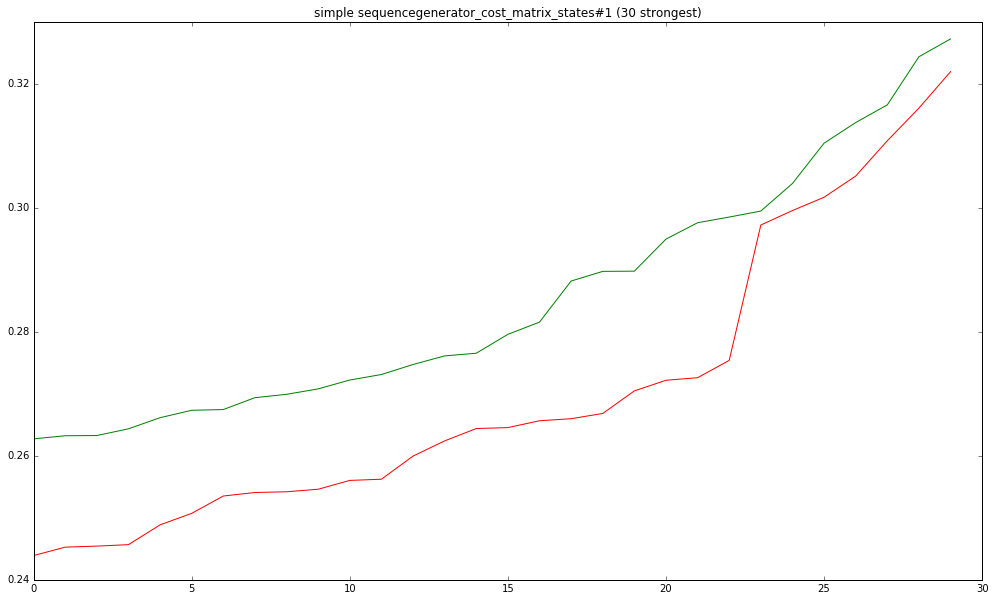
\includegraphics[width=250pt,height=150pt]{gfx/simplernn.png}
		\caption{simple recurrent, last hidden layer output (top 30 correlations)}
	\end{figure}
\end{frame}
\begin{frame}{\expv}
	\begin{figure}
		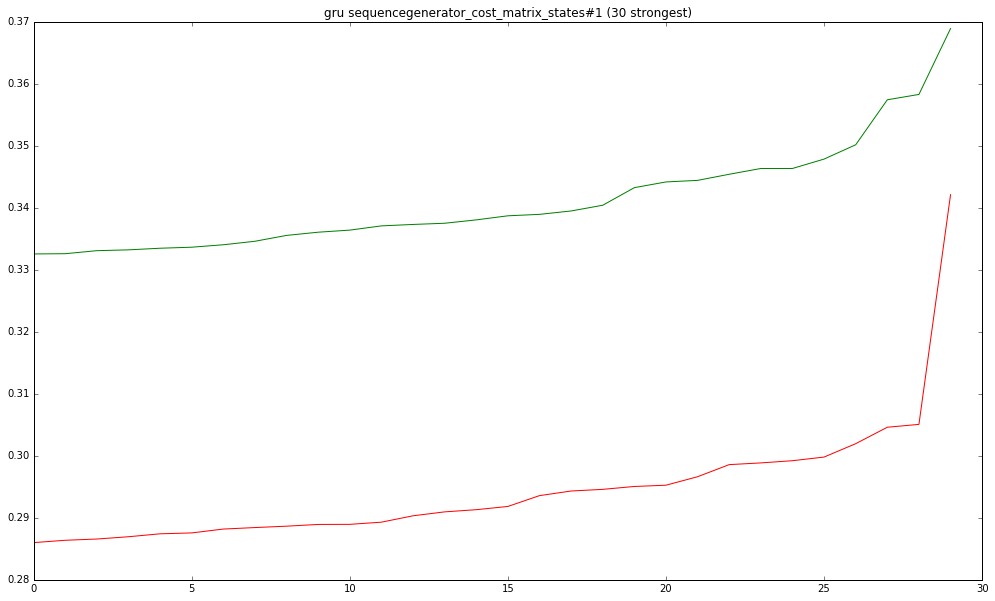
\includegraphics[width=250pt,height=150pt]{gfx/gru.png}
		\caption{gru, last hidden layer output (top 30 correlations)}
	\end{figure}
\end{frame}
\begin{frame}{\expv}
	\begin{figure}
		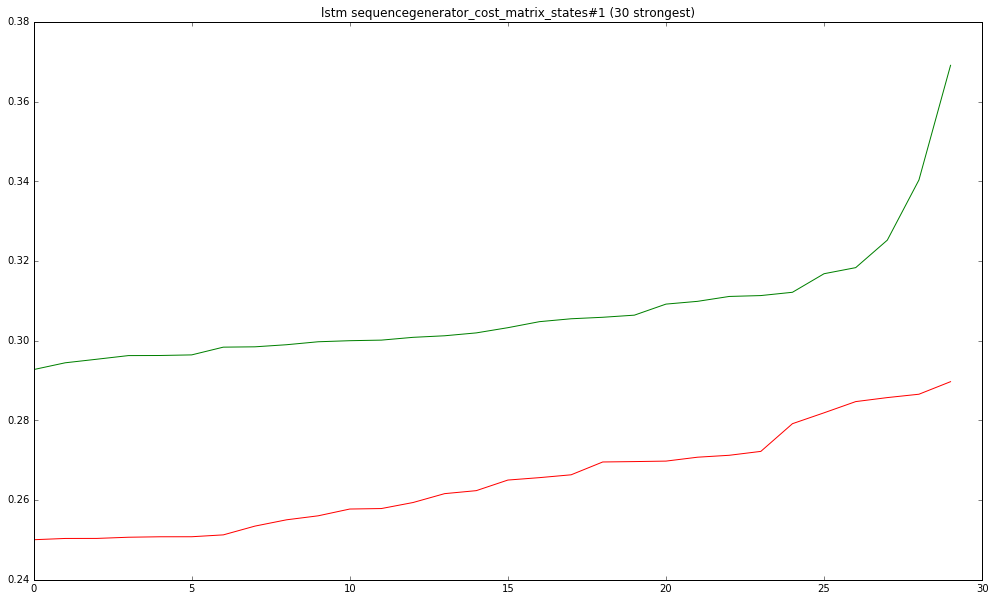
\includegraphics[width=250pt,height=150pt]{gfx/lstmstates.png}
		\caption{lstm, last hidden layer states output (top 30 correlations)}
	\end{figure}
\end{frame}
\begin{frame}{\expv}
\begin{figure}
	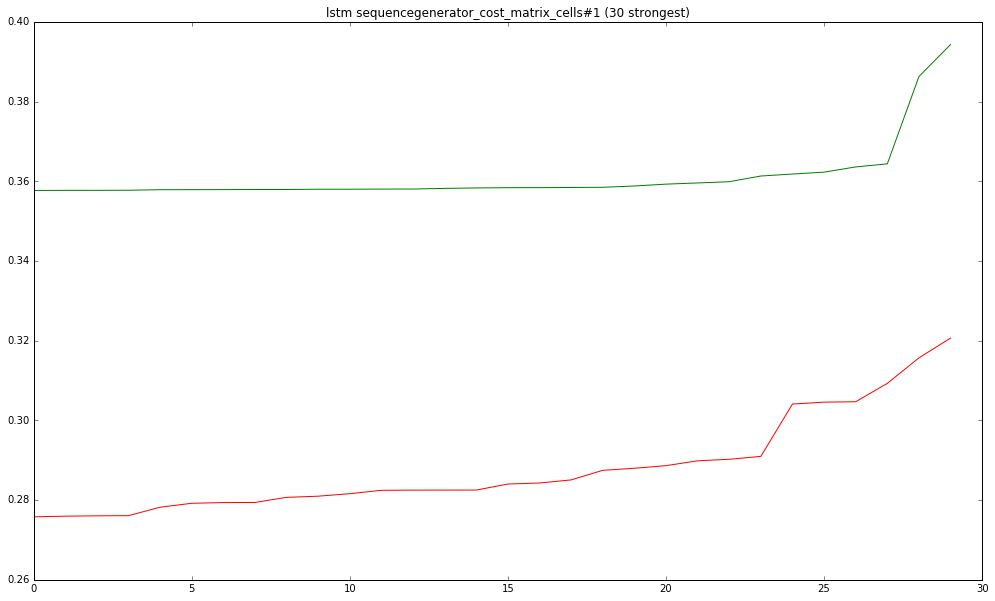
\includegraphics[width=250pt,height=150pt]{gfx/lstm.png}
	\caption{lstm, last hidden layer cells output (top 30 correlations)}
\end{figure}
\end{frame}
\begin{frame}{\expv}
	\textbf{conclusion:}
	\begin{itemize}
		\item no consistent behaviour of a single neuron over all sequences, but strong correlations of single neurons over a subset of the tested sentences
		\item do neurons \textit{cooperate} or \textit{share tasks}
		\item very unclear if these results truly represent a correlation with our phenomenon of choice
	\end{itemize}
\end{frame}
\begin{frame}{\expvi}
	\textbf{motivation:}
	\begin{itemize}
		\item we observed problems for computed correlations for both character and word level
		\item how can we still obtain the neurons showing \textit{consistency} in their behaviour (even if not over all sequences)
		\item we could plot all sentence activations and count, but well ...
		\item how can we figure out groups of neurons, that “work together“
	\end{itemize}
\end{frame}
\begin{frame}{\expvi}
	\textbf{procedure:}
	\begin{itemize}
		\item take correlation values from E5 and find $k$ strongest neurons for each sentence ($k=100$ out of 512 per layer $\times$ (cells, states))
		\item memorize these neurons for each layer
		\item cluster the sentences (which sentences have the most in common)
		\item plot some sentences to get an idea what these correlation values are about 
	\end{itemize}
\end{frame}
\begin{frame}{\expvi}
	\textbf{results:}
	\begin{itemize}
		\item the intersection of top $k$ neurons over all sentences was \textbf{empty}
		\item but \dots
	\end{itemize}
\end{frame}
\begin{frame}{\expvi}
	\begin{figure}
		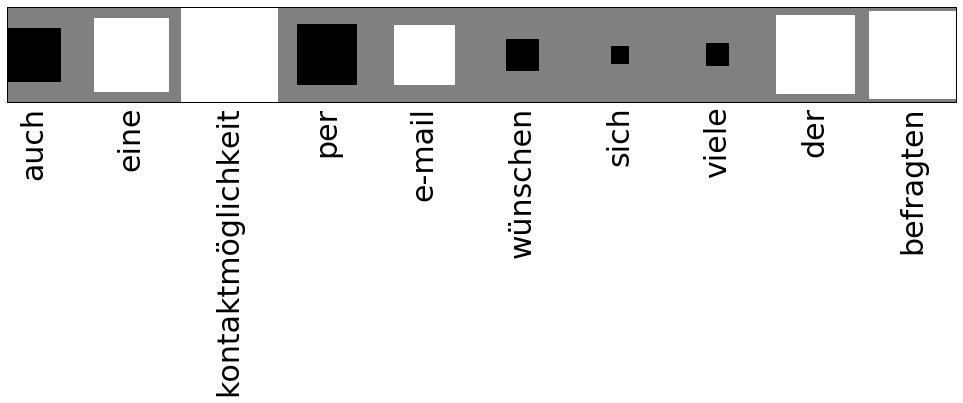
\includegraphics[width=200pt,height=100pt]{gfx/perfectneuron.png}
		\caption{LSTM, first hidden layer cells output (neuron 36)} % consitent over time
	\end{figure}
\end{frame}
\begin{frame}{\expvi}
	\begin{figure}
		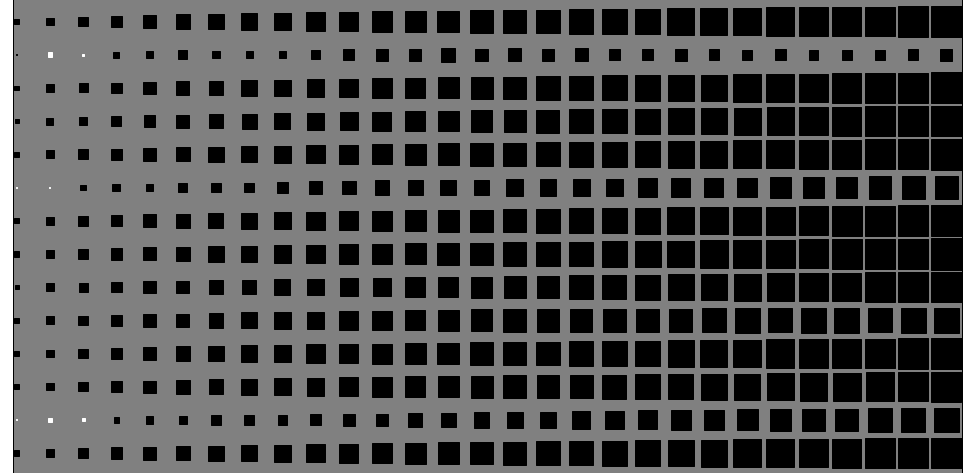
\includegraphics[width=200pt,height=100pt]{gfx/cells1length.png}
		\caption{LSTM, last hidden layer cells output (observed way more often)} % consitent over time
	\end{figure}
\end{frame}
\begin{frame}{\expvi}
	\textbf{conclusion:}
	\begin{itemize}
		\item a combined method of plotting and correlating only provided a clear answer (so far), both methods on its own seem to be insufficient
		\item indeed the computed correlations seem to have been mostly about sentence length
		\item no neuron (in the inspected areas) showed strong correlations over all sentences
		\item neurons seem to act in clusters, but these are also not constant over time
		\item there are no hints or observations, that the network captured the hierarchical relation, but somehow distributional properties of nouns with their determiners	
	\end{itemize}
\end{frame}
\begin{frame}{\expvii}
	\textbf{motivation:}
	\begin{itemize}
		\item as well as in the word-level experiment we need to explore a way to find out about neuron groups correlating with input-specific phenomena		
	\end{itemize}
	\textbf{procedure:}
	\begin{itemize}
		\item we used PCA to find the neurons explaining between 90 and 99\% of the activation variation in a 1-layered simple recurrent ($H=1024$)
		\item after that, we correlated word bounderies and sequence length on the remaining components
	\end{itemize}
\end{frame}
\begin{frame}{\expvii}
	\textbf{results:}
	\begin{itemize}
		\item dimensionality was reduced on $\approx 500$
		\item sequence length correlation decreased  
		\item word boundery correlation decreased on \texttt{0.3} (\texttt{0.6} without PCA)
	\end{itemize}
	\textbf{conclusion:}
	\begin{itemize}
		\item PCA failed
		\item we were using a linear reduction method on clearly non-linear data
		\item this motivates E10
	\end{itemize}
\end{frame}
%\begin{frame}{\expviii}
	\textbf{motivation:}
	\begin{itemize}
		\item none
	\end{itemize}
	\textbf{procedure:}
	\begin{itemize}
		\item it's a secret
	\end{itemize}
	\textbf{results:}
	\begin{itemize}
		\item 1
	\end{itemize}
	\textbf{conclusion:}
	\begin{itemize}
		\item \dots
	\end{itemize}
\end{frame}
\begin{frame}{\expix}
	\textbf{motivation:}
	\begin{itemize}
		\item activation sequences are continues signals
		\item why not using methods for signal analysis on it?
	\end{itemize}
	\textbf{procedure:}
	\begin{itemize}
		\item we decided to use an ERP signal analysis method
		\item general idea: compare averaged signals to noise to detect \textit{real events}
		\item feed the network $V$ artificial character sequences of length 2
		\item all sequences share our character of interest (COI) as first character, the second character is unique for each sequence
		\item the average of activations for these sequences is our COI's representation
		\item do the same for each other character of the vocabulary, but average over all gathered activations (noise representation)
		\item this experiment was performed for LSTM and simple recurrent on the \lk -dataset
	\end{itemize}
	\textbf{results:}
	\begin{itemize}
		\item strong differences between characters
		\item but how to interpret it?
	\end{itemize}
	\textbf{conclusion:}
	\begin{itemize}
		\item again, this method was performed for single neurons, we did not get an insight on groups of neurons which we need
	\end{itemize}
\end{frame} 
\begin{frame}{\expx}
	\textbf{motivation:}
	\begin{itemize}
		\item for non-linear data like ours (activations) with respect to our research questions, we need a non-linear method of analysis
		\item autoencoders seemded to be worth a try
		\item unfortunately this is work in progress without any results so far
	\end{itemize}
	\textbf{procedure:}
	\begin{itemize}
		\item training an autoencoder on our activation data of the \hdt~word model
		\item reduce dimensions of input down to 300 and back up again
		\item look at the inner representation of the input vectors and see what we can do with it
	\end{itemize}
	\textbf{results:}
	\begin{itemize}
		\item right now only a model for the cell outputs of a 2-layered (512, 512) LSTM exists (last layer)
		\item training parameters: input dim $512$, 1 hidden layer, $H=300$, batch-size $1000$, trained with batch normalization
		\item model performance: squared error of $\approx 26$
	\end{itemize}
\end{frame}
\begin{frame}{Review}
	\begin{itemize}
		\item searching for the one neuron doing a particular thing is a dead end
		\item correlation computation needs to be done in a contrastive manner and in the best case be added with plots to get a better impression
		\item the research questions can only be answered insufficiently and incomplete
		\item we need methods capable to deal with non-linear data
	\end{itemize}
\end{frame}
\begin{frame}{Critique}
	\begin{itemize}
		\item model checks were neglected
		\item experiment on actually checking the models predictions in the word-level case
		\item more experiments on the weight values within the network might have provided some insights
		\item we did not manage to deal with the relation between several neurons (at least until today)
	\end{itemize}
\end{frame}
%%%%%%%%%%%%%%%%%%%
%%%%%%%%%%%%%%%%%%%%%%%%%%%%%%%%%%%%%%%%%%%%%%%%%%%%%%%%%%%%%%
\begin{frame}{References}
	\bibliography{bib}
\end{frame}

\end{document}